\section{Conclusion}
We investigated the problem of recommending songs to form playlist for a given user.
A multitask learning objective was proposed that aims to provide a decent default recommendation 
if the given user is new to the system.
It makes better recommendations if the given user already has a few playlists accessible to the system.
We optimise the multitask objective from playlists of existing users by ranking songs in playlists above those are not
via solving either a constrained optimisation problem or an unconstrained one which approximates the objective but 
results in more efficient training.
Empirical experiments on two real playlist datasets show the proposed approaches work effectively.





We are aware of a few limitations of the proposed approaches, which we leave as future work.
Specifically, additional data sources (\eg music information shared on social media) or song/user 
features (\eg lyrics, user profile), as well as the sequential order of songs which could provide 
additional information to help make better recommendations.
Further, non-linear models such as deep neural networks have shown strong performance in a wide arrange of tasks,
and the linear model with sparse parameters in this work could potentially be more compact if non-linear objective were employed.

\begin{table}[h]
\centering
\caption{Performance of cold-start setting (c)}
\label{tab:perf2}
\resizebox{\columnwidth}{!}{
%\begin{table}[!h]
%\centering
%\caption{Performance of recommendation for new users}
%\label{tab:perf_plgen2}
%\resizebox{\columnwidth}{!}{
\begin{tabular}{l*{4}{c}*{4}{c}}
\toprule
\multirow{2}{*}{Method}  & \multicolumn{2}{c}{30Music} && \multicolumn{2}{c}{AotM-2011} \\ \cmidrule{2-3} \cmidrule{5-6}
                         & RPREC \textperthousand & AUC \% && RPREC \textperthousand & AUC \% \\
\midrule
Popularity Rank &           $21.4$ & $88.3$ &&                       $13.5$ & $91.8$ \\
Top10 SAGH &                $19.6$ & $54.5$ &&                       $11.5$ & $53.7$ \\
Top10 CAGH &                $19.5$ & $87.3$ &&                       $11.5$ & $89.4$ \\
Multitask Classification &  $21.0$ & $88.8$ &&                       $13.5$ & $91.6$ \\
Multitask Ranking &            N/A &    N/A &&                          N/A &    N/A \\
\bottomrule
\end{tabular}
%}
%\end{table}

}
\end{table}

\begin{figure}[h]
\centering
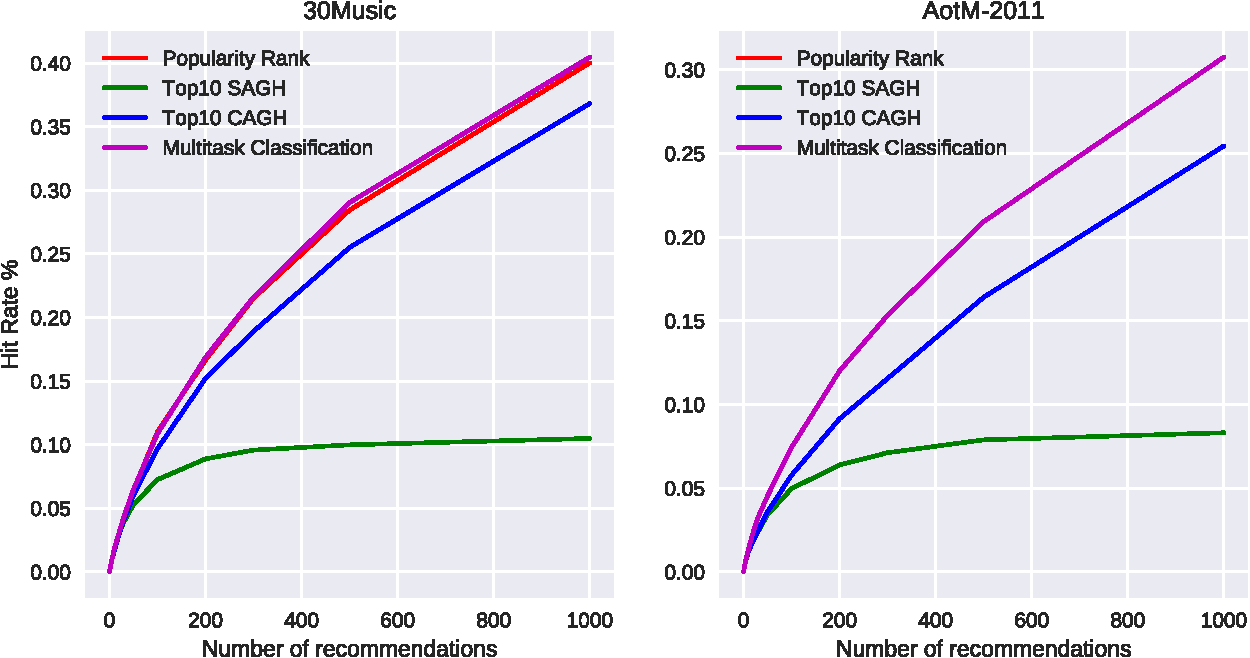
\includegraphics[width=\linewidth]{fig/hitrate2.pdf}
\caption{Hit rates of cold-start setting (c).}
\label{fig:hr2}
\end{figure}




Finally, as a remark, we want to mention the challenge of evaluating recommended results.
While metrics in information retrieval are commonly used, recommender system is more like a generative process
than a information retrieval task. Fortunately, this challenge has been noticed and been attacked in many 
ways~\cite{mcfee2011natural,mcfee2012hypergraph,schedl2017}, 
we believe that promising automatic evaluation methods that accepted by the (majority of) 
community is one premise of significant progress in music recommendation.




